\chapter{Dasar Teori}

\section{\textit{Natural Language Understanding} (NLU)}

Pemahaman bahasa alami, atau lebih dikenal dengan \textit{natural language understanding} (NLU), merupakan salah satu bagian dari pemrosesan bahasa alami atau \textit{natural language processing} (NLP). NLU adalah ranah dalam linguistik komputasional yang didedikasikan untuk memahami bahasa alami \parencite{harris2004voice}. Menurut Gartner, NLU diartikan sebagai pemahaman komputer terhadap struktur dan makna dari bahasa manusia, sehingga pengguna dapat berinteraksi dengan komputer menggunakan bahasa yang digunakan oleh pengguna.

Dasar dari NLU berasal dari enam bentuk pengetahuan yang diketahui dan dipelajari oleh manusia pada umumnya. Bentuk-bentuk pengetahuan tersebut didefinisikan sebagai berikut: \parencite{allen1995natural}

\begin{enumerate}
	\item pengetahuan fonetik dan fonologi, menyangkut pada bagaimana suara diubah menjadi susunan kata-kata. Dalam ilmu komputer, pengetahuan ini diatasi dengan menggunakan pengenalan suara (\textit{speech recognition}),
	\item pengetahuan morfologi, menyangkut pada bagaimana sebuah kata disusun dari beberapa morfem, seperti kata “terabaikan” disusun oleh tiga morfem, yaitu “ter-”, “abai”, dan “-kan”,
	\item pengetahuan sintaktis, menyangkut pada bagaimana kata-kata dapat disusun sehingga menjadi sebuah kalimat yang benar menurut tata bahasa,
	\item pengetahuan semantik, menyangkut bagaimana makna dari kata-kata disusun untuk membentuk makna dari sebuah kalimat,
	\item pengetahuan pragmatik, menyangkut bagaimana sebuah kalimat diartikan jika digunakan dalam konteks yang berbeda, dan,
	\item pengetahuan dunia, menyangkut memahami pengetahuan umum yang dipahami juga oleh pengguna untuk menjaga percakapan berjalan dengan semestinya.
\end{enumerate}

Pengetahuan yang termasuk ke dalam NLU adalah pengetahuan sintaksis, semantik, dan pragmatik.

\section{\textit{Spoken Language Understanding} (SLU)}

Pemahaman bahasa ucapan, atau \textit{spoken language understanding} (SLU), merupakan ranah yang berada di antara \textit{speech recognition}, NLP yang memanfaatkan pembelajaran mesin (\textit{machine learning}) dan kecerdasan buatan (\textit{artificial intelligence}) \parencite{tur2011spoken}. Biasanya, SLU hanya terlibat dalam dua tugas utama, yaitu klasifikasi maksud kalimat (\textit{intent classification}) dan pengisian slot (\textit{slot filling}) \parencite{goo2018slot}. Karena kedua tugas utama tersebut, SLU digunakan dalam sistem yang membutuhkan satu kalimat masukan saja dan tidak terlalu panjang.

Gambar \ref{fig:slu_early} menunjukkan rancangan sistem SLU paling awal. Sistem hanya terdiri dari \textit{automatic speech recognition} (ASR) dan NLU. Tiap komponen memiliki sumber pengetahuan masing-masing, ASR memiliki ASR KS dan NLU memiliki NLU KS. Tiap sumber pengetahuan dialirkan menuju kendali pada masing-masing proses sebelum digunakan pada proses tersebut.

\begin{figure}[H]
	\centering
	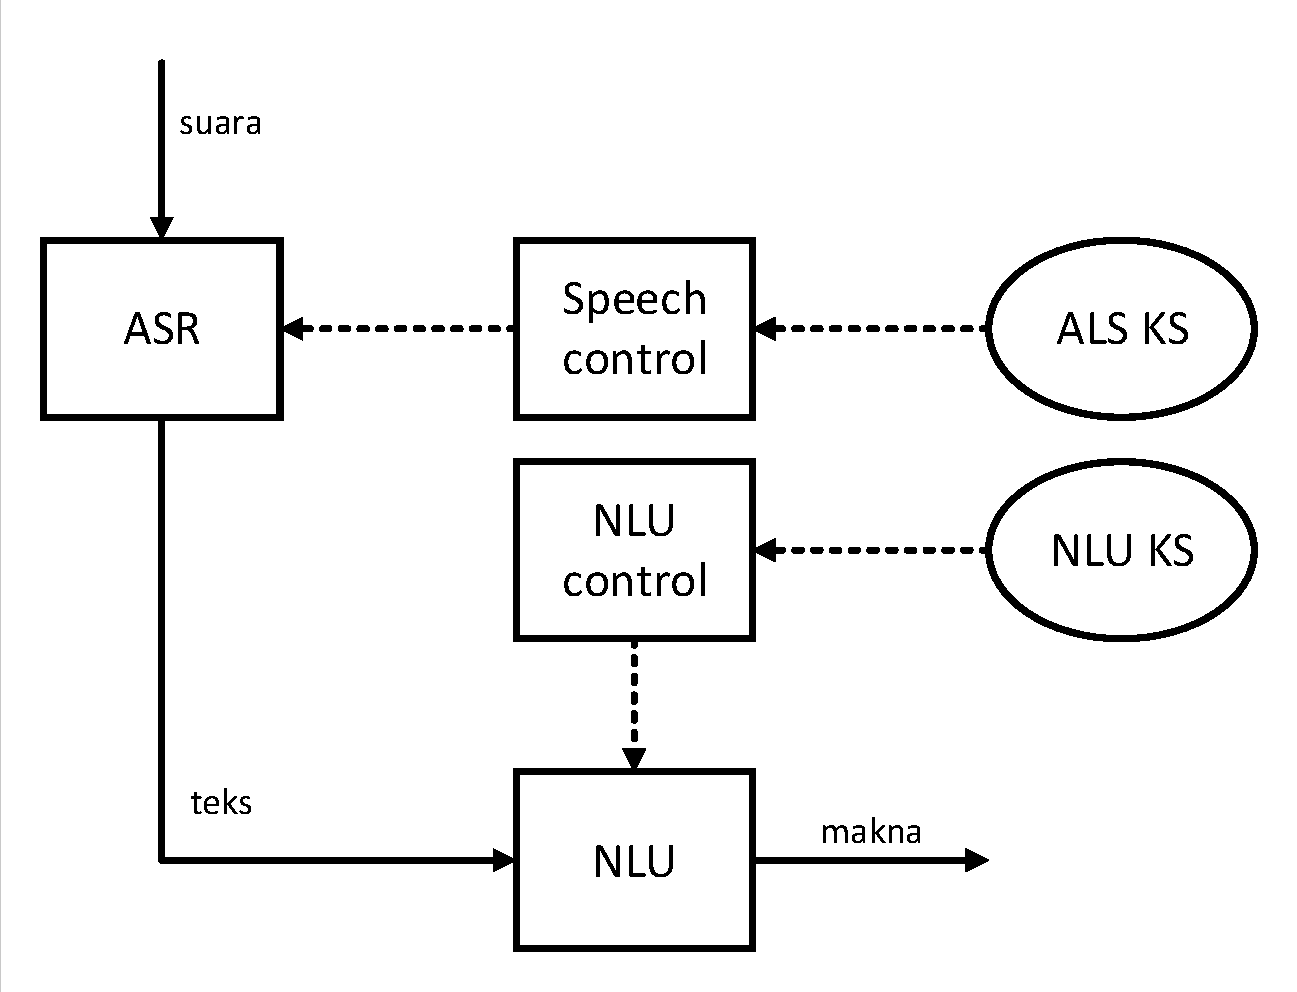
\includegraphics[width=0.5\textwidth, trim=2 2 2 2, clip]{resources/2-early_slu.pdf}
	\caption{Rancangan awal sistem SLU \parencite{tur2011spoken}}
	\label{fig:slu_early}
\end{figure}

Klasifikasi maksud kalimat berarti menentukan sebuah makna dari sebuah kalimat yang diberikan oleh pengguna. Sebagai contoh, kalimat “putarkan sebuah lagu” memiliki makna “putar media” berupa lagu. Makna tersebut kemudian diterjemahkan menjadi sebuah aksi oleh sistem. Makna kalimat bisa didapatkan dengan melihat kata-kata yang terkandung di dalam sebuah kalimat, atau melihat pola urutan kata dalam kalimat tersebut.

Pengisian slot adalah metode untuk mengambil entitas-entitas dari sebuah kalimat biasa. Beberapa aksi terkadang membutuhkan masukan parameter untuk melengkapi aksi tersebut. Masukan parameter didapatkan dari dalam kalimat yang dimasukkan oleh pengguna. Sebagai contoh, “putar lagu separuh aku dari noah” berarti pengguna menginginkan sebuah lagu diputarkan oleh sistem. Namun, permintaan pengguna menjadi lebih spesifik karena pengguna menyebutkan judul lagu beserta artis. Judul lagu adalah “separuh aku” dengan artis adalah “noah”. Metode yang dapat digunakan untuk mengambil entitas adalah melakukan pelabelan kata-kata yang menjadi entitas dengan menggunakan \textit{recurrent neural network} (RNN).

\section{\textit{Machine Learning}}

Pembelajaran mesin, atau \textit{machine learning}, adalah sebuah program komputer yang dirancang untuk belajar dari pengalaman dengan acuan berupa kelas tugas-tugas dan pengukuran performa, jika performa pada suatu tugas, yang telah diukur, diperbaiki dengan pengalaman \parencite{mitchell1997machine}. Pembelajaran mesin menggunakan data-data yang telah terkumpul untuk membentuk sebuah pola yang dapat digunakan pada data yang akan muncul.

\section{\textit{Artificial Neural Network}}

\textit{Artificial neural network} (ANN) adalah sistem komputasi yang memiliki elemen-elemen pemrosesan sederhana yang saling terhubung, yang mana dapat memproses informasi dengan respon keadaan dinamisnya kepada masukan dari luar \parencite{caudill1987neural}. ANN terdiri dari tiga jenis lapisan, yaitu lapisan masukan, lapisan tersembunyi, serta lapisan keluaran. Lapisan masukan adalah lapisan yang berisi nilai-nilai masukan berasal dari data yang telah terkumpul. Lapisan tersembunyi berisi fungsi-fungsi aktivasi yang digunakan untuk menentukan keluaran yang diinginkan oleh \textit{neural network} secara keseluruhan.

\textit{Neural network} memiliki banyak variasi untuk kondisi data yang berbeda-beda. Jenis \textit{neural network} yang sangat dasar adalah \textit{feed forward neural network}, digunakan untuk melakukan klasifikasi sederhana. Lalu terdapat 
